\def \figa { \vcenter{\hbox{ \pepob{5}{3}{{
                        "","","","",
                        "","","","",
                        "","","",""}}{{
                        "","",
                        "","",
                        "","",
                        "","",
                        "",""}}{{
                        1,1,1,1,1,
                        1,0,0,0,1,
                        1,0,0,0,1}} } }}

\def \figb { \vcenter{\hbox{  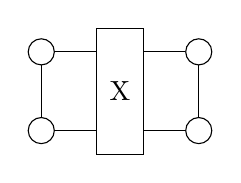
\begin{tikzpicture}[baseline=0.5]

                \def \legLength { 0.8}
                \def \radius {0.1}

                \pgfmathsetmacro{\step}{2*\radius+ \legLength} % 1
                \pgfmathsetmacro{\legpos}{\radius+\legLength} %0.9

                \node[draw, circle,radius=\radius] (L0) at (-1,0) {};
                \node[draw, circle,radius=\radius] (L1) at (-1,1) {};

                \draw (-0.3,1.3) -- (0.3,1.3) -- (0.3,-0.3) -- (-0.3,-0.3) -- cycle;

                \node[draw, circle,radius=\radius] (R0) at (1,0) {};
                \node[draw, circle,radius=\radius] (R1) at (1,1) {};

                \draw (L0) --   (L1);
                \draw (R0) --   (R1);

                \draw (L0) --   (-0.3,0);
                \draw (L1) --   (-0.3,1);

                \draw (R0) --   (0.3,0);
                \draw (R1) --   (0.3,1);

                \node[draw=none] (C0) at (0,0.5) {X};
            \end{tikzpicture}}}}

\def \figc {\vcenter{\hbox{  \begin{tikzpicture}[baseline=0.5]

                \def \legLength { 0.8}
                \def \radius {0.1}

                \pgfmathsetmacro{\step}{2*\radius+ \legLength} % 1
                \pgfmathsetmacro{\legpos}{\radius+\legLength} %0.9

                \node[draw=none, circle,radius=\radius] (L0) at (-1,0) {};
                \node[draw=none, circle,radius=\radius] (L1) at (-1,1) {};

                \draw (-0.3,1.3) -- (0.3,1.3) -- (0.3,-0.3) -- (-0.3,-0.3) -- cycle;

                \node[draw=none, circle,radius=\radius] (R0) at (1,0) {};
                \node[draw=none, circle,radius=\radius] (R1) at (1,1) {};

                \draw (L0) --   (-0.3,0);
                \draw (L1) --   (-0.3,1);

                \draw (R0) --   (0.3,0);
                \draw (R1) --   (0.3,1);

                \node[draw=none] (C0) at (0,0.5) {X};
            \end{tikzpicture} }} }

\def \figd {\vcenter{\hbox{  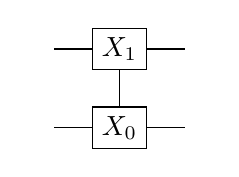
\begin{tikzpicture}[baseline=0.5]

                \def \legLength { 0.8}
                \def \radius {0.1}

                \pgfmathsetmacro{\step}{2*\radius+ \legLength} % 1
                \pgfmathsetmacro{\legpos}{\radius+\legLength} %0.9

                \node[draw=none, circle,radius=\radius] (L0) at (-1,0) {};
                \node[draw=none, circle,radius=\radius] (L1) at (-1,1) {};

                \node[draw] (C0) at (0,0) {$X_0$};
                \node[draw] (C1) at (0,1) {$X_1$};

                \node[draw=none, circle,radius=\radius] (R0) at (1,0) {};
                \node[draw=none, circle,radius=\radius] (R1) at (1,1) {};

                \draw (L0) --   (C0);
                \draw (L1) --   (C1);

                \draw (R0) --   (C0);
                \draw (R1) --   (C1);

                \draw (C1) --   (C0);
            \end{tikzpicture} }}}

%%%%%%%%%%%%%%%%%%%%%%55

\def \pepoat {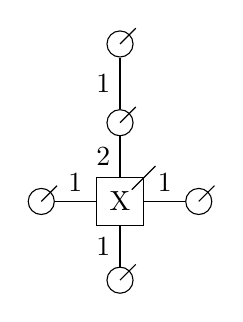
\begin{tikzpicture}[baseline=0.5]

        \def \legLength { 0.8}
        \def \radius {0.1}

        \pgfmathsetmacro{\step}{2*\radius+ \legLength} % 1
        \pgfmathsetmacro{\legpos}{\radius+\legLength} %0.9

        \node[draw,minimum size=0.6cm] (O0) at (0,0) {X};
        \draw (0.15,0.15) -- ++(0.3,0.3);

        \node[draw, circle,radius=\radius] (L1) at (-1,0) {};
        %\node[draw, circle,radius=\radius] (L2) at (-2,0) {};
        %\node[draw, circle,radius=\radius] (L3) at (-3,0) {};

        \node[draw, circle,radius=\radius] (U1) at (0,1) {};
        \node[draw, circle,radius=\radius] (U2) at (0,2) {};

        \node[draw, circle,radius=\radius] (D1) at (0,-1) {};

        \node[draw, circle,radius=\radius] (R1) at (1,0) {};

        \draw (O0) -- node [above] {1}  (L1);
        %\draw (L2) -- node [above] {2}  (L1);
        %\draw (L2) -- node [above] {1}  (L3);

        \draw (O0) -- node [left] {2}  (U1);
        \draw (U2) -- node [left] {1}  (U1);

        \draw (O0) -- node [above] {1}  (R1);

        \draw (O0) --  node [left] {1} (D1);

        \draw (L1.center) -- ++(0.2,0.2);
        %\draw (L2.center) -- ++(0.2,0.2);
        %\draw (L3.center) -- ++(0.2,0.2);
        \draw (U1.center) -- ++(0.2,0.2);
        \draw (U2.center) -- ++(0.2,0.2);
        \draw (R1.center) -- ++(0.2,0.2);
        \draw (D1.center) -- ++(0.2,0.2);

    \end{tikzpicture}}

\def \blockat {  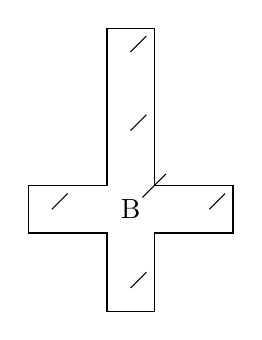
\begin{tikzpicture}[baseline=0.5]

        \def \legLength { 0.8}
        \def \radius {0.1}

        \pgfmathsetmacro{\step}{2*\radius+ \legLength} % 1
        \pgfmathsetmacro{\legpos}{\radius+\legLength} %0.9

        %\node[draw=none] (O0) at (0,0) {};
        \node[draw=none,minimum size=0.6cm] (O0) at (0,0) {B};
        \draw (0.15,0.15) -- ++(0.3,0.3);

        \node[draw=none] (L1) at (-1,0) {};
        %\node[draw=none] (L2) at (-2,0) {};
        %\node[draw=none] (L3) at (-3,0) {};

        \node[draw=none] (U1) at (0,1) {};
        \node[draw=none] (U2) at (0,2) {};

        \node[draw=none] (D1) at (0,-1) {};

        \node[draw=none] (R1) at (1,0) {};

        %\draw (O0.center) -- ++(0.45,0.45);
        \draw (L1.center) -- ++(0.2,0.2);
        %\draw (L2.center) -- ++(0.2,0.2);
        %\draw (L3.center) -- ++(0.2,0.2);
        \draw (U1.center) -- ++(0.2,0.2);
        \draw (U2.center) -- ++(0.2,0.2);
        \draw (R1.center) -- ++(0.2,0.2);
        \draw (D1.center) -- ++(0.2,0.2);

        \draw (-1.3,0.3)--(-0.3,0.3) -- (-0.3,2.3)--(0.3,2.3)
        -- (0.3,0.3) -- (1.3,0.3) -- (1.3,-0.3) -- (0.3,-0.3)
        -- (0.3,-1.3) -- (-0.3, -1.3) -- (-0.3,-0.3) -- (-1.3,-0.3) -- cycle;

    \end{tikzpicture}}

\def \pepobt {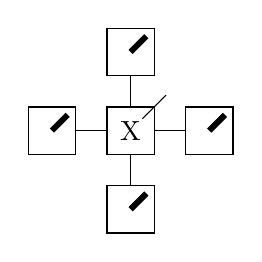
\begin{tikzpicture}[baseline=0.5]

        \def \legLength { 0.8}
        \def \radius {0.1}

        \pgfmathsetmacro{\step}{2*\radius+ \legLength} % 1
        \pgfmathsetmacro{\legpos}{\radius+\legLength} %0.9

        %\node[draw, circle, radius=\radius] (O0) at (0,0) {};
        \node[draw,minimum size=0.6cm] (O0) at (0,0) {X};
        \draw (0.15,0.15) -- ++(0.3,0.3);

        \node[draw, minimum size=0.6cm] (L1) at (-1,0) {};
        \node[draw, minimum size=0.6cm] (U1) at (0,1) {};
        \node[draw, minimum size=0.6cm] (D1) at (0,-1) {};
        \node[draw, minimum size=0.6cm] (R1) at (1,0) {};

        \draw (O0) -- (L1);
        \draw (O0) -- (U1);
        \draw (O0) -- (R1);
        \draw (O0) -- (D1);

        %\draw(O0.center) -- ++(0.2,0.2);
        \draw[line width=0.75mm]  (L1.center) -- ++(0.2,0.2);
        \draw[line width=0.75mm] (U1.center) -- ++(0.2,0.2);
        \draw[line width=0.75mm] (R1.center) -- ++(0.2,0.2);
        \draw[line width=0.75mm] (D1.center) -- ++(0.2,0.2);

    \end{tikzpicture} }

\def \blockbt {   \begin{tikzpicture}[baseline=0.5]

        \def \legLength { 0.8}
        \def \radius {0.1}

        \pgfmathsetmacro{\step}{2*\radius+ \legLength} % 1
        \pgfmathsetmacro{\legpos}{\radius+\legLength} %0.9

        %\node[draw=none] (O0) at (0,0) {};
        \node[draw=none,minimum size=0.6cm] (O0) at (0,0) {B};
        \draw (0.15,0.15) -- ++(0.3,0.3);

        \node[draw=none] (L1) at (-1,0) {};
        \node[draw=none] (L2) at (-2,0) {};
        \node[draw=none] (L3) at (-3,0) {};

        \node[draw=none] (U1) at (0,1) {};
        \node[draw=none] (U2) at (0,2) {};

        \node[draw=none] (D1) at (0,-1) {};

        \node[draw=none] (R1) at (1,0) {};

        %\draw (O0.center) -- ++(0.45,0.45);
        \draw[line width=0.75mm] (L3.center) -- ++(0.2,0.2);
        \draw[line width=0.75mm] (U2.center) -- ++(0.2,0.2);
        \draw[line width=0.75mm] (R1.center) -- ++(0.2,0.2);
        \draw[line width=0.75mm] (D1.center) -- ++(0.2,0.2);

        \draw (-3.3,0.3)--(-0.3,0.3) -- (-0.3,2.3)--(0.3,2.3)
        -- (0.3,0.3) -- (1.3,0.3) -- (1.3,-0.3) -- (0.3,-0.3)
        -- (0.3,-1.3) -- (-0.3, -1.3) -- (-0.3,-0.3) -- (-3.3,-0.3) -- cycle;

    \end{tikzpicture} }

\def \pepoct { 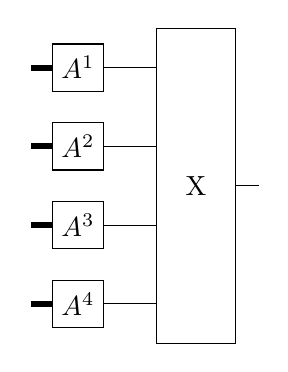
\begin{tikzpicture}[baseline=0.5]
        \draw (0,2.5)-- (0,-1.5) -- (1,-1.5)-- (1,2.5) -- cycle;

        \node[draw=none] (x)  at (0.5,0.5) {X};

        \node[draw, minimum size=0.6cm] (n1)  at (-1,2) {$A^1$};
        \node[draw, minimum size=0.6cm] (n2)  at (-1,1) {$A^2$};
        \node[draw, minimum size=0.6cm] (n3)  at (-1,0) {$A^3$};
        \node[draw, minimum size=0.6cm] (n4)  at (-1,-1) {$A^4$};

        \draw (n1) -- node [above] {} (0,2);
        \draw (n2) -- node [above] {} (0,1);
        \draw (n3) -- node [above] {} (0,0);
        \draw (n4) -- node [above] {} (0,-1);

        \draw[line width=0.75mm] (n1) -- ++(-0.6,0) ;
        \draw[line width=0.75mm] (n2) -- ++(-0.6,0) ;
        \draw[line width=0.75mm] (n3) -- ++(-0.6,0) ;
        \draw[line width=0.75mm] (n4) -- ++(-0.6,0);

        \draw (1,0.5) -- (1.3,0.5)  ;

    \end{tikzpicture} }

\def \blockct { \begin{tikzpicture}[baseline=3]
        \draw (0,2.5)-- (0,-1.5) -- (1,-1.5)-- (1,2.5) -- cycle;

        \node[draw=none] (x)  at (0.5,0.5) {B};

        \draw[line width=0.75mm] (-0.3,2)  node [left] {}  -- (0,2) ;
        \draw[line width=0.75mm] (-0.3,1)  node [left] {} -- (0,1);
        \draw[line width=0.75mm] (-0.3,0)  node [left] {} -- (0,0);
        \draw[line width=0.75mm] (-0.3,-1)  node [left] {} -- (0,-1);

        \draw (1,0.5) -- (1.3,0.5)  node [right] {} ;

    \end{tikzpicture} }

\def \pepocta { 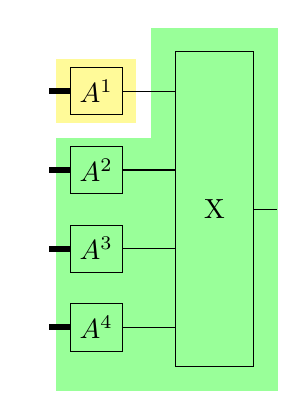
\begin{tikzpicture}[baseline=0.5]

        \path[draw, fill=yellow!40,color=yellow!40] (-1.5,2.4) -- (-0.5,2.4)--(-0.5,1.6)--(-1.5,1.6)-- cycle;

        \path[draw, fill=green!40,color=green!40] (-1.5,1.4) -- (-0.3,1.4)--(-0.3,2.8)--(1.3,2.8)-- (1.3,-1.8) -- (-1.5 ,-1.8) -- cycle;

        \draw (0,2.5)-- (0,-1.5) -- (1,-1.5)-- (1,2.5) -- cycle;

        \node[draw=none] (x)  at (0.5,0.5) {X};

        \node[draw, minimum size=0.6cm] (n1)  at (-1,2) {$A^1$};
        \node[draw, minimum size=0.6cm] (n2)  at (-1,1) {$A^2$};
        \node[draw, minimum size=0.6cm] (n3)  at (-1,0) {$A^3$};
        \node[draw, minimum size=0.6cm] (n4)  at (-1,-1) {$A^4$};

        \draw (n1) -- node [above] {} (0,2);
        \draw (n2) -- node [above] {} (0,1);
        \draw (n3) -- node [above] {} (0,0);
        \draw (n4) -- node [above] {} (0,-1);

        \draw[line width=0.75mm] (n1) -- ++(-0.6,0) node [left] {};
        \draw[line width=0.75mm] (n2) -- ++(-0.6,0) node [left] {};
        \draw[line width=0.75mm] (n3) -- ++(-0.6,0) node [left] {};
        \draw[line width=0.75mm] (n4) -- ++(-0.6,0) node [left] {};

        \draw (1,0.5) -- (1.3,0.5)  ;

    \end{tikzpicture} }

\def \blockcta { 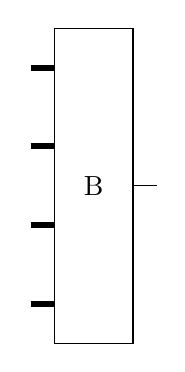
\begin{tikzpicture}[baseline=3]
        \draw (0,2.5)-- (0,-1.5) -- (1,-1.5)-- (1,2.5) -- cycle;

        \node[draw=none] (x)  at (0.5,0.5) {B};

        \draw[line width=0.75mm] (-0.3,2)   -- (0,2) ;
        \draw[line width=0.75mm] (-0.3,1)  -- (0,1);
        \draw[line width=0.75mm] (-0.3,0)   -- (0,0);
        \draw[line width=0.75mm] (-0.3,-1)  -- (0,-1);

        \draw (1,0.5) -- (1.3,0.5)   ;

    \end{tikzpicture} }

\def \pepoctb { 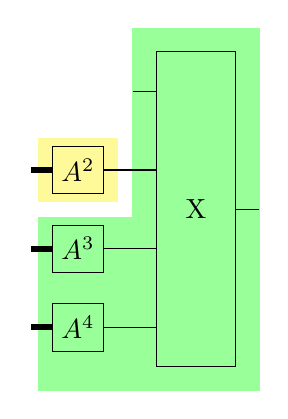
\begin{tikzpicture}[baseline=0.5]

        \path[draw, fill=yellow!40,color=yellow!40] (-1.5,1.4) -- (-0.5,1.4)--(-0.5,0.6)--(-1.5,0.6)-- cycle;

        \path[draw, fill=green!40,color=green!40] (-1.5,0.4) -- (-0.3,0.4)--(-0.3,2.8)--(1.3,2.8)-- (1.3,-1.8) -- (-1.5 ,-1.8) -- cycle;

        \draw (0,2.5)-- (0,-1.5) -- (1,-1.5)-- (1,2.5) -- cycle;

        \node[draw=none] (x)  at (0.5,0.5) {X};

        \node[draw, minimum size=0.6cm] (n2)  at (-1,1) {$A^2$};
        \node[draw, minimum size=0.6cm] (n3)  at (-1,0) {$A^3$};
        \node[draw, minimum size=0.6cm] (n4)  at (-1,-1) {$A^4$};

        \draw (-0.3,2) -- node [above] {} (0,2);
        \draw (n2) -- node [above] {} (0,1);
        \draw (n3) -- node [above] {} (0,0);
        \draw (n4) -- node [above] {} (0,-1);

        \draw[line width=0.75mm] (n2) -- ++(-0.6,0) ;
        \draw[line width=0.75mm] (n3) -- ++(-0.6,0) ;
        \draw[line width=0.75mm] (n4) -- ++(-0.6,0) ;

        \draw (1,0.5) -- (1.3,0.5)  ;

    \end{tikzpicture} }

\def \blockctb { 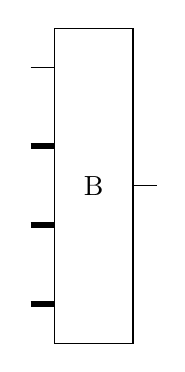
\begin{tikzpicture}[baseline=3]
        \draw (0,2.5)-- (0,-1.5) -- (1,-1.5)-- (1,2.5) -- cycle;

        \node[draw=none] (x)  at (0.5,0.5) {B};

        \draw (-0.3,2)    -- (0,2) ;
        \draw[line width=0.75mm] (-0.3,1)   -- (0,1);
        \draw[line width=0.75mm] (-0.3,0)   -- (0,0);
        \draw[line width=0.75mm] (-0.3,-1)  -- (0,-1);

        \draw (1,0.5) -- (1.3,0.5)  ;

    \end{tikzpicture} }

\def \pepoctc { 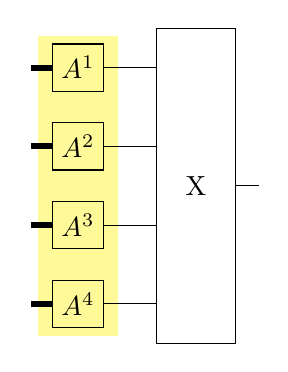
\begin{tikzpicture}[baseline=0.5]

        \path[draw, fill=yellow!40,color=yellow!40] (-1.5,2.4) -- (-0.5,2.4)--(-0.5,-1.4)--(-1.5,-1.4)-- cycle;

        \draw (0,2.5)-- (0,-1.5) -- (1,-1.5)-- (1,2.5) -- cycle;

        \node[draw=none] (x)  at (0.5,0.5) {X};

        \node[draw, minimum size=0.6cm] (n1)  at (-1,2) {$A^1$};
        \node[draw, minimum size=0.6cm] (n2)  at (-1,1) {$A^2$};
        \node[draw, minimum size=0.6cm] (n3)  at (-1,0) {$A^3$};
        \node[draw, minimum size=0.6cm] (n4)  at (-1,-1) {$A^4$};

        \draw (n1) -- node [above] {} (0,2);
        \draw (n2) -- node [above] {} (0,1);
        \draw (n3) -- node [above] {} (0,0);
        \draw (n4) -- node [above] {} (0,-1);

        \draw[line width=0.75mm] (n1) -- ++(-0.6,0) ;
        \draw[line width=0.75mm] (n2) -- ++(-0.6,0) ;
        \draw[line width=0.75mm] (n3) -- ++(-0.6,0) ;
        \draw[line width=0.75mm] (n4) -- ++(-0.6,0) ;

        \draw (1,0.5) -- (1.3,0.5)  ;

    \end{tikzpicture} }

\def \pepoctd{ 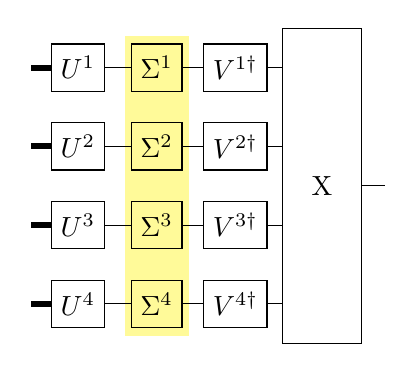
\begin{tikzpicture}[baseline=0.5]

        \path[draw, fill=yellow!40,color=yellow!40] (-2.0,2.4) -- (-1.2,2.4)--(-1.2,-1.4)--(-2.0,-1.4)-- cycle;

        \draw (0,2.5)-- (0,-1.5) -- (1,-1.5)-- (1,2.5) -- cycle;

        \node[draw=none] (x)  at (0.5,0.5) {X};

        \node[draw, minimum size=0.6cm] (n11)  at (-2.6,2) {$U^1$};
        \node[draw, minimum size=0.6cm] (n12)  at (-1.6,2) {$\Sigma^1$};
        \node[draw, minimum size=0.6cm] (n13)  at (-0.6,2) {$V^{1 \dagger}$};

        \node[draw, minimum size=0.6cm] (n21)  at (-2.6,1) {$U^2$};
        \node[draw, minimum size=0.6cm] (n22)  at (-1.6,1) {$\Sigma^2$};
        \node[draw, minimum size=0.6cm] (n23)  at (-0.6,1) {$V^{2 \dagger}$};

        \node[draw, minimum size=0.6cm] (n31)  at (-2.6,0) {$U^3$};
        \node[draw, minimum size=0.6cm] (n32)  at (-1.6,0) {$\Sigma^3$};
        \node[draw, minimum size=0.6cm] (n33)  at (-0.6,0) {$V^{3 \dagger}$};

        \node[draw, minimum size=0.6cm] (n41)  at (-2.6,-1) {$U^4$};
        \node[draw, minimum size=0.6cm] (n42)  at (-1.6,-1) {$\Sigma^4$};
        \node[draw, minimum size=0.6cm] (n43)  at (-0.6,-1) {$V^{4 \dagger}$};

        \draw (n12) --  (n13);
        \draw (n11) --  (n12);

        \draw (n22) --  (n23);
        \draw (n21) --  (n22);

        \draw (n32) --  (n33);
        \draw (n31) --  (n32);

        \draw (n42) --  (n43);
        \draw (n41) --  (n42);

        \draw (n13) -- node [above] {} (0,2);
        \draw (n23) -- node [above] {} (0,1);
        \draw (n33) -- node [above] {} (0,0);
        \draw (n43) -- node [above] {} (0,-1);

        \draw[line width=0.75mm] (n11) -- ++(-0.6,0) ;
        \draw[line width=0.75mm] (n21) -- ++(-0.6,0) ;
        \draw[line width=0.75mm] (n31) -- ++(-0.6,0) ;
        \draw[line width=0.75mm] (n41) -- ++(-0.6,0) ;

        \draw (1,0.5) -- (1.3,0.5)  ;

    \end{tikzpicture} }
%%%%%%%%%%%%%%%%

\def \pa { 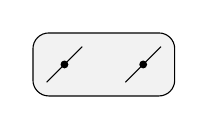
\begin{tikzpicture}[clust/.style = {rounded corners= 0.2 cm, fill=gray!10}]

        \def \e {0.40}

        \def \radius {0.1}
        \def \ll {0.35}

        \draw[clust] (1-\e,1-\e)--(1-\e,1+\e)--(2+\e,1+\e)--(2+\e,1-\e)--cycle;

        \foreach \x in {1,2}
            {
                \foreach \y in {1}
                    {
                        \pgfmathtruncatemacro{\s}{\x*10+\y   }

                        \fill (\x,\y) circle (0.05cm);

                        \pgfmathsetmacro{\pp}{   \x+\ll }
                        \pgfmathsetmacro{\pm}{   \x-\ll  }

                        \pgfmathsetmacro{\kp}{   \y+\ll  }
                        \pgfmathsetmacro{\km}{   \y-\ll  }

                        \node (Op\s) at (\pp,\kp) {};
                        \node (Om\s) at (\pm,\km) {};

                        \draw (\x,\y)  --  (Op\s);
                        \draw  (\x,\y) --  (Om\s);
                    }
            }

    \end{tikzpicture}}

\def \pb { 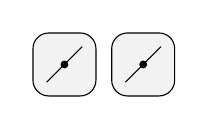
\begin{tikzpicture}[clust/.style = {rounded corners= 0.2 cm, fill=gray!10}]

        \def \e {0.40}

        \def \radius {0.1}
        \def \ll {0.35}

        \draw[clust] (1-\e,1-\e)--(1-\e,1+\e)--(1+\e,1+\e)--(1+\e,1-\e)--cycle;
        \draw[clust] (2-\e,1-\e)--(2-\e,1+\e)--(2+\e,1+\e)--(2+\e,1-\e)--cycle;

        %\draw[clust] (1-\e,1-\e)--(1-\e,1+\e)--(2+\e,1+\e)--(2+\e,1-\e)--cycle;

        \foreach \x in {1,2}
            {
                \foreach \y in {1}
                    {
                        \pgfmathtruncatemacro{\s}{\x*10+\y   }

                        \fill (\x,\y) circle (0.05cm);

                        \pgfmathsetmacro{\pp}{   \x+\ll }
                        \pgfmathsetmacro{\pm}{   \x-\ll  }

                        \pgfmathsetmacro{\kp}{   \y+\ll  }
                        \pgfmathsetmacro{\km}{   \y-\ll  }

                        \node (Op\s) at (\pp,\kp) {};
                        \node (Om\s) at (\pm,\km) {};

                        \draw (\x,\y)  --  (Op\s);
                        \draw  (\x,\y) --  (Om\s);
                    }
            }

    \end{tikzpicture}}

\def \pc { 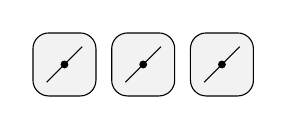
\begin{tikzpicture}[clust/.style = {rounded corners= 0.2 cm, fill=gray!10}]

        \def \e {0.40}

        \def \radius {0.1}
        \def \ll {0.35}

        \draw[clust] (1-\e,1-\e)--(1-\e,1+\e)--(1+\e,1+\e)--(1+\e,1-\e)--cycle;
        \draw[clust] (2-\e,1-\e)--(2-\e,1+\e)--(2+\e,1+\e)--(2+\e,1-\e)--cycle;
        \draw[clust] (3-\e,1-\e)--(3-\e,1+\e)--(3+\e,1+\e)--(3+\e,1-\e)--cycle;

        %\draw[clust] (1-\e,1-\e)--(1-\e,1+\e)--(2+\e,1+\e)--(2+\e,1-\e)--cycle;

        \foreach \x in {1,2,3}
            {
                \foreach \y in {1}
                    {
                        \pgfmathtruncatemacro{\s}{\x*10+\y   }

                        \fill (\x,\y) circle (0.05cm);

                        \pgfmathsetmacro{\pp}{   \x+\ll }
                        \pgfmathsetmacro{\pm}{   \x-\ll  }

                        \pgfmathsetmacro{\kp}{   \y+\ll  }
                        \pgfmathsetmacro{\km}{   \y-\ll  }

                        \node (Op\s) at (\pp,\kp) {};
                        \node (Om\s) at (\pm,\km) {};

                        \draw (\x,\y)  --  (Op\s);
                        \draw  (\x,\y) --  (Om\s);
                    }
            }

    \end{tikzpicture}}

\def \pca { 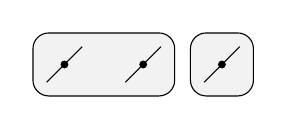
\begin{tikzpicture}[clust/.style = {rounded corners= 0.2 cm, fill=gray!10}]

        \def \e {0.40}

        \def \radius {0.1}
        \def \ll {0.35}

        \draw[clust] (1-\e,1-\e)--(1-\e,1+\e)--(2+\e,1+\e)--(2+\e,1-\e)--cycle;
        \draw[clust] (3-\e,1-\e)--(3-\e,1+\e)--(3+\e,1+\e)--(3+\e,1-\e)--cycle;

        %\draw[clust] (1-\e,1-\e)--(1-\e,1+\e)--(2+\e,1+\e)--(2+\e,1-\e)--cycle;

        \foreach \x in {1,2,3}
            {
                \foreach \y in {1}
                    {
                        \pgfmathtruncatemacro{\s}{\x*10+\y   }

                        \fill (\x,\y) circle (0.05cm);

                        \pgfmathsetmacro{\pp}{   \x+\ll }
                        \pgfmathsetmacro{\pm}{   \x-\ll  }

                        \pgfmathsetmacro{\kp}{   \y+\ll  }
                        \pgfmathsetmacro{\km}{   \y-\ll  }

                        \node (Op\s) at (\pp,\kp) {};
                        \node (Om\s) at (\pm,\km) {};

                        \draw (\x,\y)  --  (Op\s);
                        \draw  (\x,\y) --  (Om\s);
                    }
            }

    \end{tikzpicture}}

\def \pcb { 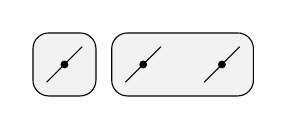
\begin{tikzpicture}[clust/.style = {rounded corners= 0.2 cm, fill=gray!10}]

        \def \e {0.40}

        \def \radius {0.1}
        \def \ll {0.35}

        \draw[clust] (1-\e,1-\e)--(1-\e,1+\e)--(1+\e,1+\e)--(1+\e,1-\e)--cycle;
        \draw[clust] (2-\e,1-\e)--(2-\e,1+\e)--(3+\e,1+\e)--(3+\e,1-\e)--cycle;

        %\draw[clust] (1-\e,1-\e)--(1-\e,1+\e)--(2+\e,1+\e)--(2+\e,1-\e)--cycle;

        \foreach \x in {1,2,3}
            {
                \foreach \y in {1}
                    {
                        \pgfmathtruncatemacro{\s}{\x*10+\y   }

                        \fill (\x,\y) circle (0.05cm);

                        \pgfmathsetmacro{\pp}{   \x+\ll }
                        \pgfmathsetmacro{\pm}{   \x-\ll  }

                        \pgfmathsetmacro{\kp}{   \y+\ll  }
                        \pgfmathsetmacro{\km}{   \y-\ll  }

                        \node (Op\s) at (\pp,\kp) {};
                        \node (Om\s) at (\pm,\km) {};

                        \draw (\x,\y)  --  (Op\s);
                        \draw  (\x,\y) --  (Om\s);
                    }
            }

    \end{tikzpicture}}

\def \pcc { 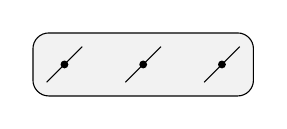
\begin{tikzpicture}[clust/.style = {rounded corners= 0.2 cm, fill=gray!10}]

        \def \e {0.40}

        \def \radius {0.1}
        \def \ll {0.35}

        \draw[clust] (1-\e,1-\e)--(1-\e,1+\e)--(3+\e,1+\e)--(3+\e,1-\e)--cycle;

        %\draw[clust] (1-\e,1-\e)--(1-\e,1+\e)--(2+\e,1+\e)--(2+\e,1-\e)--cycle;

        \foreach \x in {1,2,3}
            {
                \foreach \y in {1}
                    {
                        \pgfmathtruncatemacro{\s}{\x*10+\y   }

                        \fill (\x,\y) circle (0.05cm);

                        \pgfmathsetmacro{\pp}{   \x+\ll }
                        \pgfmathsetmacro{\pm}{   \x-\ll  }

                        \pgfmathsetmacro{\kp}{   \y+\ll  }
                        \pgfmathsetmacro{\km}{   \y-\ll  }

                        \node (Op\s) at (\pp,\kp) {};
                        \node (Om\s) at (\pm,\km) {};

                        \draw (\x,\y)  --  (Op\s);
                        \draw  (\x,\y) --  (Om\s);
                    }
            }

    \end{tikzpicture}}

\def \paa {
\begin{tikzpicture}[clust/.style = {rounded corners= 0.2 cm, fill=gray!10}]

        \def \e {0.40}

        \def \radius {0.1}
        \def \ll {0.35}

        \draw[clust] (1-\e,1-\e)--(1-\e,1+\e)--(1+\e,1+\e)--(1+\e,1-\e)--cycle;

        \foreach \x in {1}
            {
                \foreach \y in {1}
                    {
                        \pgfmathtruncatemacro{\s}{\x*10+\y   }

                        \fill (\x,\y) circle (0.05cm);

                        \pgfmathsetmacro{\pp}{   \x+\ll }
                        \pgfmathsetmacro{\pm}{   \x-\ll  }

                        \pgfmathsetmacro{\kp}{   \y+\ll  }
                        \pgfmathsetmacro{\km}{   \y-\ll  }

                        \node (Op\s) at (\pp,\kp) {};
                        \node (Om\s) at (\pm,\km) {};

                        \draw (\x,\y)  --  (Op\s);
                        \draw  (\x,\y) --  (Om\s);
                    }
            }

    \end{tikzpicture}}

%%%%%%%%%%%%%%%
\def \crossloop{ 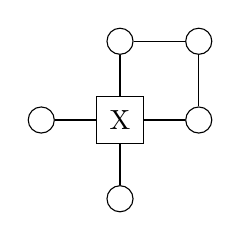
\begin{tikzpicture}[baseline=0.5]

        \def \legLength { 0.8}
        \def \radius {0.1}

        \pgfmathsetmacro{\step}{2*\radius+ \legLength} % 1
        \pgfmathsetmacro{\legpos}{\radius+\legLength} %0.9

        \node[draw, circle,radius=\radius] (L0) at (-1,0) {};

        \draw (-0.3,0.3) -- (0.3,0.3) -- (0.3,-0.3) -- (-0.3,-0.3) -- cycle;

        \node[draw, circle,radius=\radius] (R0) at (1,0) {};
        \node[draw, circle,radius=\radius] (R1) at (1,1) {};

        \node[draw, circle,radius=\radius] (U) at (0,1) {};
        \node[draw, circle,radius=\radius] (D) at (0,-1) {};

        \draw (R0) --   (R1);

        \draw (L0) --   (-0.3,0);

        \draw (R0) --   (0.3,0);
        \draw (U) --   (0,0.3);
        \draw (D) --   (0,-0.3);
        \draw (R1) --   (U);

        \node[draw=none] (C0) at (0,0) {X};
    \end{tikzpicture} }

%%%%%%%%%%%%%%
\def \clustFullA {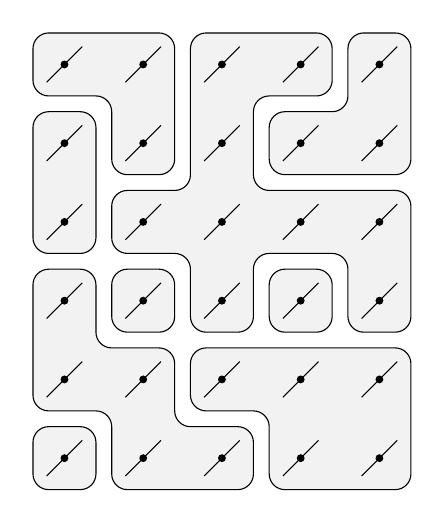
\begin{tikzpicture}[clust/.style = {rounded corners= 0.2 cm, fill=gray!10}]

        \def \e {0.40}

        \draw[clust] (1-\e,1-\e)--(1-\e,1+\e)--(1+\e,1+\e)--(1+\e,1-\e)--cycle;
        %\draw (,)--(,)--(,)--(,)--cycle;
        \draw[clust ] (3-\e,2+\e) -- (5+\e,2+\e) -- (5+\e,1-\e) -- (4-\e, 1-\e) -- (4-\e, 2-\e)-- (3-\e, 2-\e)--cycle;
        \draw[clust ] (1-\e,3+\e)--(1+\e, 3+\e)-- (1+\e,2+\e) -- (2+\e,2+\e) -- (2+\e,1+\e)--(3+\e,1+\e)-- (3+\e,1-\e)--(2-\e,1-\e)--(2-\e,2-\e) -- (1-\e,2-\e)--cycle;
        \draw[clust] (2-\e, 4-\e) -- (2-\e,4+ \e) -- (3-\e, 4+\e) -- (3-\e,6+ \e) -- (4+\e,6+ \e) -- (4+\e, 6-\e) -- (3+\e, 6-\e) -- (3+\e,4+ \e) -- (5+\e,4+ \e) -- (5+\e,3- \e) -- (5-\e,3- \e) -- (5-\e, 4-\e) -- (3+\e, 4-\e) -- (3+\e,3- \e) -- (3-\e, 3-\e)-- (3-\e, 4-\e) --cycle;
        \draw[clust] (4-\e,5-\e)--(4-\e,5+\e)--(5-\e,5+\e)--(5-\e,6+\e)--(5+\e,6+\e)--(5+\e,5-\e)--cycle;
        \draw[clust] (2-\e,3-\e)--(2-\e,3+\e)--(2+\e,3+\e)--(2+\e,3-\e)--cycle;
        \draw[clust] (4-\e,3-\e)--(4-\e,3+\e)--(4+\e,3+\e)--(4+\e,3-\e)--cycle;
        \draw[clust] (1-\e,4- \e)--(1-\e, 5+ \e)--(1+\e, 5+\e)--(1+\e, 4-\e)--cycle;
        \draw[clust] (1-\e, 6-\e)--(1-\e,6+ \e)--(2+\e, 6+ \e)--(2+\e,5- \e)--(2-\e, 5- \e)--(2-\e,6- \e)--cycle;

        \def \sz {5};

        \def \radius {0.1}
        \def \ll {0.35}

        \foreach \x in {1,2,..., 5}
            {
                \foreach \y in {1,2,..., 6}
                    {
                        \pgfmathtruncatemacro{\s}{\x*10+\y   }

                        \fill (\x,\y) circle (0.05cm);

                        %\node[draw=none] (O\s) at (\x,\y) {};

                        \pgfmathsetmacro{\pp}{   \x+\ll }
                        \pgfmathsetmacro{\pm}{   \x-\ll  }

                        \pgfmathsetmacro{\kp}{   \y+\ll  }
                        \pgfmathsetmacro{\km}{   \y-\ll  }

                        \node (Op\s) at (\pp,\kp) {};
                        \node (Om\s) at (\pm,\km) {};

                        \draw (\x,\y)  --  (Op\s);
                        \draw  (\x,\y) --  (Om\s);

                    }
            }

    \end{tikzpicture} }

\def \clustFullB {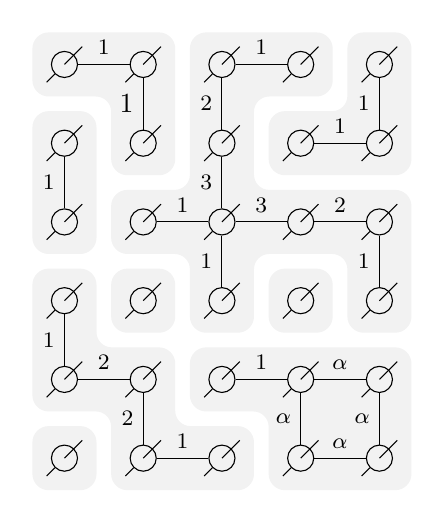
\begin{tikzpicture}[clust/.style = {rounded corners= 0.2 cm,  ,fill=gray!10, color=gray!10 }]

        \def \e {0.40}

        \draw[clust] (1-\e,1-\e)--(1-\e,1+\e)--(1+\e,1+\e)--(1+\e,1-\e)--cycle;
        %\draw (,)--(,)--(,)--(,)--cycle;
        \draw[clust ] (3-\e,2+\e) -- (5+\e,2+\e) -- (5+\e,1-\e) -- (4-\e, 1-\e) -- (4-\e, 2-\e)-- (3-\e, 2-\e)--cycle;
        \draw[clust ] (1-\e,3+\e)--(1+\e, 3+\e)-- (1+\e,2+\e) -- (2+\e,2+\e) -- (2+\e,1+\e)--(3+\e,1+\e)-- (3+\e,1-\e)--(2-\e,1-\e)--(2-\e,2-\e) -- (1-\e,2-\e)--cycle;
        \draw[clust] (2-\e, 4-\e) -- (2-\e,4+ \e) -- (3-\e, 4+\e) -- (3-\e,6+ \e) -- (4+\e,6+ \e) -- (4+\e, 6-\e) -- (3+\e, 6-\e) -- (3+\e,4+ \e) -- (5+\e,4+ \e) -- (5+\e,3- \e) -- (5-\e,3- \e) -- (5-\e, 4-\e) -- (3+\e, 4-\e) -- (3+\e,3- \e) -- (3-\e, 3-\e)-- (3-\e, 4-\e) --cycle;
        \draw[clust] (4-\e,5-\e)--(4-\e,5+\e)--(5-\e,5+\e)--(5-\e,6+\e)--(5+\e,6+\e)--(5+\e,5-\e)--cycle;
        \draw[clust] (2-\e,3-\e)--(2-\e,3+\e)--(2+\e,3+\e)--(2+\e,3-\e)--cycle;
        \draw[clust] (4-\e,3-\e)--(4-\e,3+\e)--(4+\e,3+\e)--(4+\e,3-\e)--cycle;
        \draw[clust] (1-\e,4- \e)--(1-\e, 5+ \e)--(1+\e, 5+\e)--(1+\e, 4-\e)--cycle;
        \draw[clust] (1-\e, 6-\e)--(1-\e,6+ \e)--(2+\e, 6+ \e)--(2+\e,5- \e)--(2-\e, 5- \e)--(2-\e,6- \e)--cycle;

        \def \sz {5};

        \def \radius {0.1}
        \def \ll {0.35}

        \foreach \x in {1,2,..., 5}
            {
                \foreach \y in {1,2,..., 6}
                    {
                        \pgfmathtruncatemacro{\s}{\x*10+\y   }

                        \node[draw, circle, radius = \radius ] (O\s) at (\x,\y) {};

                        \pgfmathsetmacro{\pp}{   \x+\ll }
                        \pgfmathsetmacro{\pm}{   \x-\ll  }

                        \pgfmathsetmacro{\kp}{   \y+\ll  }
                        \pgfmathsetmacro{\km}{   \y-\ll  }

                        \node (Op\s) at (\pp,\kp) {};
                        \node (Om\s) at (\pm,\km) {};

                        \draw (O\s.center)  --  (Op\s);
                        \draw (Om\s) --  (O\s);

                    }
            }

        %vertical
        \draw (O12) -- node [left] {\footnotesize 1} (O13);
        \draw (O14) -- node [left] {\footnotesize 1} (O15);

        \draw (O21) -- node [left] {\footnotesize 2} (O22);
        \draw (O25) -- node [left] {1} (O26);

        \draw (O33) -- node [left] {\footnotesize 1} (O34);
        \draw (O34) -- node [left] {\footnotesize 3} (O35);
        \draw (O35) -- node [left] {\footnotesize 2} (O36);

        \draw (O41) -- node [left] {\footnotesize $\alpha$} (O42);

        \draw (O51) -- node [left] {\footnotesize $\alpha$} (O52);
        \draw (O53) -- node [left] {\footnotesize 1} (O54);
        \draw (O55) -- node [left] {\footnotesize 1} (O56);

        %horizontal

        \draw (O21) -- node [above] {\footnotesize 1} (O31);
        \draw (O41) -- node [above] {\footnotesize $\alpha$} (O51);

        \draw (O12) -- node [above] {\footnotesize 2} (O22);
        \draw (O32) -- node [above] {\footnotesize 1} (O42);
        \draw (O42) -- node [above] {\footnotesize $\alpha$} (O52);

        \draw (O24) -- node [above] {\footnotesize 1} (O34);
        \draw (O34) -- node [above] {\footnotesize 3} (O44);
        \draw (O44) -- node [above] {\footnotesize 2} (O54);

        \draw (O45) -- node [above] {\footnotesize 1} (O55);

        \draw (O16) -- node [above] {\footnotesize 1} (O26);
        \draw (O36) -- node [above] {\footnotesize 1} (O46);

    \end{tikzpicture}}

%%%%%%%%%%%%%%%%%%%
\def \mpograph {\mpo{5}{{"Tr","$\chi$",,,,}}{{"$i_1$","$i_2$",,"$i_n$","-"}}{{"-","-",,"-","-"}}{{0,0,1,0,0}}{{"C", "C",,"C","M" }}}

\def \ctens { \begin{tikzpicture}[baseline={0.5cm-0.5*height("$=$")}]

        \draw (-3,-0) rectangle (1,1)  [add reference=C]   ;
        \node  at (C center) {C};

        \node (N1)  at  (-2.5,1.6) {$i_1$};
        \node (N2)  at  (-1.5,1.6) {$i_2$};
        \node  at  (-.5,1.25) {...};
        \node  (N3) at  (.5,1.6) {$i_n$};

        \draw    (N1) -- (N1 |-  C north);
        \draw    (N2) -- (N2 |-  C north);
        \draw    (N3) -- (N3 |-  C north);

    \end{tikzpicture} }
